\definecolor{networkblue}{RGB}{42,95,170}
\definecolor{networkteal}{RGB}{32,139,145}
\definecolor{networkcyan}{RGB}{50,168,190}
\definecolor{networkgreen}{RGB}{75,150,93}
\definecolor{networkamber}{RGB}{226,137,38}

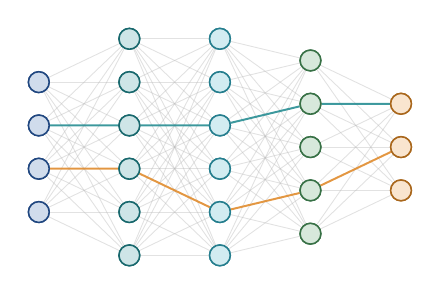
\begin{tikzpicture}[
  neuron/.style={
    circle,
    draw=#1!75!black,
    fill=#1!22,
    line width=0.55pt,
    minimum size=7.5pt,
    inner sep=0pt
  },
  connection/.style={
    line width=0.32pt,
    draw=gray!55,
    opacity=0.42
  },
  active connection/.style={
    line width=0.72pt,
    opacity=0.85
  }
]
\def\layersep{1.15}
\def\nodesep{0.55}

\foreach \i in {1,...,4} {
  \pgfmathsetmacro{\y}{0.825 - (\i - 1) * \nodesep}
  \node[neuron=networkblue] (L0-\i) at (0,\y) {};
}

\foreach \i in {1,...,6} {
  \pgfmathsetmacro{\y}{1.375 - (\i - 1) * \nodesep}
  \node[neuron=networkteal] (L1-\i) at (\layersep,\y) {};
  \node[neuron=networkcyan] (L2-\i) at (2*\layersep,\y) {};
}

\foreach \i in {1,...,5} {
  \pgfmathsetmacro{\y}{1.1 - (\i - 1) * \nodesep}
  \node[neuron=networkgreen] (L3-\i) at (3*\layersep,\y) {};
}

\foreach \i in {1,...,3} {
  \pgfmathsetmacro{\y}{0.55 - (\i - 1) * \nodesep}
  \node[neuron=networkamber] (L4-\i) at (4*\layersep,\y) {};
}

\foreach \i in {1,...,4} {
  \foreach \j in {1,...,6} {
    \draw[connection] (L0-\i) -- (L1-\j);
  }
}

\foreach \i in {1,...,6} {
  \foreach \j in {1,...,6} {
    \draw[connection] (L1-\i) -- (L2-\j);
  }
}

\foreach \i in {1,...,6} {
  \foreach \j in {1,...,5} {
    \draw[connection] (L2-\i) -- (L3-\j);
  }
}

\foreach \i in {1,...,5} {
  \foreach \j in {1,...,3} {
    \draw[connection] (L3-\i) -- (L4-\j);
  }
}

\draw[active connection, draw=networkteal] (L0-2) -- (L1-3) -- (L2-3) -- (L3-2) -- (L4-1);
\draw[active connection, draw=networkamber] (L0-3) -- (L1-4) -- (L2-5) -- (L3-4) -- (L4-2);

\foreach \i in {1,...,4} {
  \node[neuron=networkblue] at (L0-\i) {};
}

\foreach \i in {1,...,6} {
  \node[neuron=networkteal] at (L1-\i) {};
  \node[neuron=networkcyan] at (L2-\i) {};
}

\foreach \i in {1,...,5} {
  \node[neuron=networkgreen] at (L3-\i) {};
}

\foreach \i in {1,...,3} {
  \node[neuron=networkamber] at (L4-\i) {};
}
\end{tikzpicture}
